% =====================================================================
%  Analisi Matematica II — Lezione 3 (seguito)
%  Inizio delle serie di funzioni (la prima parte della lezione è in
%  discontinuita-e-criteri-di-cauchy.tex).
%  Frammento da includere con \input; richiede amsmath, amssymb, graphicx.
% =====================================================================

% [0:29:08]
\section{Serie di funzioni}

% [0:32:00]
\subsection{Definizione}

\paragraph{Definizione.} Sia $f_n:I\subseteq\mathbb{R}\to\mathbb{R}$ per ogni
$n\in\mathbb{N}$. Si chiama \emph{serie di funzioni} di termine generale $f_n(x)$, e si
scrive
\begin{equation}
\sum_{n=1}^{+\infty}f_n(x),
\end{equation}
la successione di funzioni delle \emph{somme parziali}
\begin{equation}
S_1(x)=f_1(x),\qquad S_2(x)=f_1(x)+f_2(x)=S_1(x)+f_2(x),\qquad\dots
\end{equation}
e, in generale,
\begin{equation}
S_n(x)=S_{n-1}(x)+f_n(x).
\end{equation}
Si dice che la serie \emph{converge puntualmente} alla somma $S(x)$ in $I$ se
$S_n\to S$ puntualmente in $I$; si dice che \emph{converge uniformemente} a $S(x)$ in $I$
se $S_n\rightrightarrows S$ in $I$.

\paragraph{Osservazione.} Come per le successioni, la convergenza uniforme implica quella
puntuale.

% [0:29:08]
\paragraph{In aula.} La teoria delle serie di funzioni è, nelle parole della docente,
``povera'': a differenza delle serie numeriche, dove si dispone di molti criteri, lo studio
di una serie di funzioni generica può essere un esercizio molto complesso. Il motivo è che
la convergenza uniforme richiede di conoscere $S$, e già in Analisi I le uniche serie di
cui si sapeva calcolare la somma erano le geometriche e le telescopiche. L'obiettivo vero
del corso non sono le serie generiche ma le \emph{serie di potenze}, cioè quelle che hanno
la forma del polinomio di Taylor: la definizione generale serve per arrivarci.

% [0:30:38]
\paragraph{In aula.} I tipi di convergenza saranno quattro: puntuale, uniforme, assoluta e
totale. Inoltre l'insieme $I$ è scritto come sottoinsieme di $\mathbb{R}$, ma fra poco si
lavorerà con sottoinsiemi di $\mathbb{R}^2$: la definizione si trasporta senza modifiche.

% [0:34:47]
\paragraph{In aula.} Rispetto ad Analisi I non si parla più di \emph{carattere} della
serie: qui si tratta soltanto di stabilire se c'è convergenza e di che tipo. Dire che la
serie converge puntualmente significa che, fissato $x$, la serie numerica corrispondente
converge.

% [0:36:15]
\subsection{Esempio 1: la serie geometrica}

\paragraph{Esempio.} Si studi la convergenza puntuale e uniforme di
\begin{equation}
\sum_{n=0}^{+\infty}x^n,\qquad x\in\mathbb{R}.
\end{equation}

\emph{Convergenza puntuale.} È la serie geometrica di ragione $x$: converge puntualmente
se e solo se $|x|<1$, con somma
\begin{equation}
S(x)=\frac{1}{1-x},\qquad x\in\,]-1,1[\,.
\end{equation}

\emph{Convergenza uniforme in $]-1,1[$.} Dalla formula della progressione geometrica,
$S_n(x)=\dfrac{1-x^{\,n+1}}{1-x}$, e quindi
\begin{equation}
\sup_{]-1,1[}\big|S_n(x)-S(x)\big|
=\sup_{]-1,1[}\left|\frac{1-x^{\,n+1}}{1-x}-\frac{1}{1-x}\right|
=\sup_{]-1,1[}\frac{|x|^{\,n+1}}{1-x}=+\infty ,
\end{equation}
perché per $x\to1^-$ il numeratore tende a $1$ e il denominatore a $0^+$. Dunque
\[
S_n\to S\ \text{puntualmente in }]-1,1[,\qquad S_n\not\rightrightarrows S\ \text{in }]-1,1[.
\]

\emph{Come recuperare l'uniformità.} Come per le successioni, ci si allontana dagli
estremi: per ogni $r$ con $0<r<1$ si ha
\begin{equation}
\sup_{[-r,r]}\big|S_n(x)-S(x)\big|\le\frac{r^{\,n+1}}{1-r}\longrightarrow 0,
\end{equation}
quindi la convergenza è uniforme su ogni compatto $\{|x|\le r\}\subset\,]-1,1[$.

% [0:40:04]
\paragraph{In aula.} La serie geometrica di Analisi I era già, senza dirlo, una serie di
funzioni: bastava chiamare $x$ la ragione $q$. È il primo esempio da tenere presente anche
perché $x^n$ è già il prototipo del termine di una serie di potenze.

% [0:43:56]
\paragraph{In aula.} Il motivo per cui il sup esplode è tutto nel denominatore: per quanto
$|x|^{\,n+1}$ diventi piccolo, avvicinandosi a $1$ il denominatore $1-x$ manda il rapporto
all'infinito. L'intervallo aperto è il problema; appena ci si mette in un compatto più
piccolo, tutto funziona.

% [0:50:30]
\subsection{Esempio 2: una serie a segni alterni}

\paragraph{Esempio.} Si studi la convergenza puntuale, uniforme e assoluta di
\begin{equation}
\sum_{n=1}^{+\infty}(-1)^n\,\frac{x^2+n}{n^2},\qquad x\in[-1,1].
\end{equation}

\emph{Convergenza puntuale.} Si applica il criterio di Leibniz, fissato $x$. Posto
\begin{equation}
a_n(x)=\frac{x^2+n}{n^2}=\frac{x^2}{n^2}+\frac{1}{n},
\end{equation}
si vede subito che $a_n(x)>0$, che $a_n(x)$ è decrescente in $n$ (entrambi gli addendi lo
sono, e la monotonia richiesta è in $n$, non in $x$) e che $a_n(x)\to0$. Quindi la serie
converge puntualmente per ogni $x\in[-1,1]$.

\emph{Convergenza uniforme.} Non conosciamo $S$, ma per le serie a segni alterni viene in
aiuto la \emph{stima del resto}: $|S_n(x)-S(x)|\le a_{n+1}(x)$. Allora
\begin{equation}
\sup_{[-1,1]}\big|S_n(x)-S(x)\big|\le\sup_{[-1,1]}a_{n+1}(x)
=\sup_{[-1,1]}\frac{x^2+n+1}{(n+1)^2}=\frac{n+2}{(n+1)^2}\longrightarrow0,
\end{equation}
dove il sup si calcola in $x=\pm1$ perché $x$ varia in un compatto. Dunque la serie
converge uniformemente in $[-1,1]$.

% [0:51:32]
\paragraph{In aula.} La stima del resto — che in Analisi I poteva sembrare un dettaglio —
è esattamente ciò che rende le serie a segni alterni comode anche in Analisi II: maggiora
$|S_n-S|$ senza richiedere di conoscere $S$, e riporta il problema allo studio di una
successione. Se il primo termine trascurato non tende a zero uniformemente, però, il
criterio non dice nulla e ci si ferma.

% [0:55:22]
\subsection{Convergenza assoluta}

\paragraph{Definizione.} Sia $f_n:I\subseteq\mathbb{R}\to\mathbb{R}$. La serie
$\sum_{n=1}^{+\infty}f_n$ \emph{converge assolutamente} in $I$ se converge puntualmente la
serie dei moduli
\begin{equation}
\sum_{n=1}^{+\infty}|f_n(x)| .
\end{equation}

\paragraph{Esempio.} La serie dell'Esempio 2 non converge assolutamente: per ogni
$x\in[-1,1]$
\begin{equation}
\sum_{n=1}^{+\infty}\frac{x^2+n}{n^2}\ \ge\ \sum_{n=1}^{+\infty}\frac{1}{n},
\end{equation}
che diverge. Si ha quindi convergenza uniforme \emph{senza} convergenza assoluta.

% [0:56:58]
\paragraph{In aula.} Questo esempio servirà ancora: mostra che fra convergenza assoluta e
convergenza uniforme non c'è alcun legame, in nessuno dei due versi. La serie dei moduli,
qui, si comporta in sostanza come la serie armonica generalizzata.

% [0:59:23]
\subsection{Criteri di Cauchy per le serie di funzioni}

Si ottengono scrivendo i criteri di Cauchy per la successione delle somme parziali,
osservando che
\[
S_{n+p}(x)-S_n(x)=f_{n+1}(x)+\dots+f_{n+p}(x)
\]
è il \emph{resto} della serie.

\paragraph{Criterio di Cauchy (convergenza puntuale).}
Sia $f_n:I\subseteq\mathbb{R}\to\mathbb{R}$ per ogni $n\in\mathbb{N}$:
$\sum_{n=1}^{+\infty}f_n(x)$
converge puntualmente in $I$ se e solo se
\begin{equation}
\forall x\in I,\ \forall\varepsilon>0\ \ \exists\,\nu_{x,\varepsilon}:\quad
\big|f_{n+1}(x)+\dots+f_{n+p}(x)\big|<\varepsilon
\qquad\forall p\in\mathbb{N},\ \forall n>\nu_{x,\varepsilon}.
\end{equation}

\paragraph{Criterio di Cauchy (convergenza uniforme).}
Sia $f_n:I\subseteq\mathbb{R}\to\mathbb{R}$ per ogni $n\in\mathbb{N}$:
$\sum_{n=1}^{+\infty}f_n(x)$
converge uniformemente in $I$ se e solo se
\begin{equation}
\forall\varepsilon>0\ \ \exists\,\nu_{\varepsilon}:\quad
\big|f_{n+1}(x)+\dots+f_{n+p}(x)\big|<\varepsilon
\qquad\forall p\in\mathbb{N},\ \forall n>\nu_{\varepsilon},\ \forall x\in I.
\end{equation}

% [1:01:27]
\paragraph{In aula.} Non c'è niente da dimostrare: sono i criteri di Cauchy per le
successioni, applicati alle somme parziali. Il primo è addirittura il criterio di Analisi I
scritto punto per punto. Si introducono adesso perché da essi escono immediatamente le
condizioni di convergenza.

% [1:02:56]
\subsection{Condizione necessaria per la convergenza uniforme}

\paragraph{Teorema.} Sia $f_n:I\subseteq\mathbb{R}\to\mathbb{R}$ per ogni $n$. Se
$\sum_{n=1}^{+\infty}f_n(x)$ converge uniformemente in $I$, allora
\begin{equation}
f_n\rightrightarrows 0\quad\text{in }I .
\end{equation}

\paragraph{Dimostrazione.} Si applica il criterio di Cauchy uniforme con $p=1$: resta
$|f_{n+1}(x)|<\varepsilon$ per ogni $n>\nu_\varepsilon$ e per ogni $x\in I$, che è
esattamente la definizione di $f_n\rightrightarrows0$. $\blacksquare$

% [1:02:56]
\paragraph{In aula.} È lo stesso meccanismo di Analisi I, dove si scriveva
$a_n=S_n-S_{n-1}$ per dedurre che il termine generale di una serie convergente tende a
zero; qui, non potendo usare quell'argomento nella versione uniforme, lo si ottiene
direttamente da Cauchy. La versione puntuale (il termine generale tende a zero
puntualmente) è ancora Analisi I, applicata $x$ per $x$.

% [1:08:07]
\subsection{Convergenza totale e criterio di Weierstrass}

\paragraph{Definizione (convergenza totale).} Sia
$f_n:I\subseteq\mathbb{R}\to\mathbb{R}$. La serie $\sum_{n=1}^{+\infty}f_n(x)$ converge
\emph{totalmente} in $I$ se esiste una successione numerica $M_n>0$ tale che
\begin{enumerate}
  \item $|f_n(x)|\le M_n$ per ogni $n\in\mathbb{N}$ e per ogni $x\in I$;
  \item la serie numerica $\sum_{n=1}^{+\infty}M_n$ converge.
\end{enumerate}

\paragraph{Osservazione.} Valgono le implicazioni
\begin{equation}
\text{TOTALE}\ \Longrightarrow\ \text{ASSOLUTA}\ \Longrightarrow\ \text{PUNTUALE},
\end{equation}
la prima perché $\sum|f_n(x)|$ è maggiorata da $\sum M_n$, la seconda per il criterio di
Analisi I.

% [1:08:07]
\paragraph{In aula.} L'idea della definizione è semplice: non potendo calcolare
$\sup_I|S_n-S|$, si maggiora la serie dei moduli con una serie numerica convergente, cioè
con qualcosa che \emph{non dipende da $x$}. Non basta la convergenza assoluta: serve una
maggiorazione uniforme rispetto a $x$.

% [1:12:16]
\paragraph{In aula.} Il numero $M_n$ non è altro che il $m_n=\sup_I|f_n(x)|$ che si usava
per la convergenza uniforme (con funzione limite nulla). Non è obbligatorio prendere
proprio il sup: va bene qualunque maggiorante più semplice da calcolare, come si fa negli
esercizi cercando una maggiorazione asintotica comoda.

% [1:14:55]
\paragraph{Teorema (criterio di Weierstrass).} Sia
$f_n:I\subseteq\mathbb{R}\to\mathbb{R}$ per ogni $n$. Se $\sum_{n=1}^{+\infty}f_n$
converge totalmente in $I$, allora converge uniformemente in $I$.

\paragraph{Dimostrazione.} Per ipotesi esiste $M_n>0$ con $|f_n(x)|\le M_n$ per ogni $n$ e
ogni $x\in I$, e $\sum M_n$ converge. Per il criterio di Cauchy applicato alla serie
\emph{numerica} $\sum M_n$,
\[
\forall\varepsilon>0\ \exists\,\nu:\quad M_{n+1}+\dots+M_{n+p}<\varepsilon
\qquad\forall p\in\mathbb{N},\ \forall n>\nu,
\]
e $\nu$ non dipende da $x$ perché i $M_n$ sono numeri. Allora, per la disuguaglianza
triangolare,
\begin{equation}
\big|f_{n+1}(x)+\dots+f_{n+p}(x)\big|\le|f_{n+1}(x)|+\dots+|f_{n+p}(x)|
\le M_{n+1}+\dots+M_{n+p}<\varepsilon
\end{equation}
per ogni $p\in\mathbb{N}$, ogni $n>\nu$ e \emph{ogni} $x\in I$. Vale dunque il criterio di
Cauchy per la convergenza uniforme, e la serie converge uniformemente in $I$.
$\blacksquare$

% [1:21:06]
\paragraph{In aula.} Il criterio di Cauchy viene usato due volte e nei due versi opposti:
in un verso per le serie numeriche (da $\sum M_n$ convergente si ricava la condizione di
Cauchy), nell'altro per le serie di funzioni (dalla condizione di Cauchy si ricava la
convergenza uniforme). È l'unico strumento che permette di dimostrare la convergenza
uniforme senza conoscere la somma.

% [1:16:17]
\paragraph{In aula.} Lo schema delle implicazioni si può leggere come due binari
(figura~\ref{fig:09}): dalla convergenza totale si arriva alla puntuale passando o per
l'assoluta o per l'uniforme, ma fra assoluta e uniforme non c'è alcun legame. Da qui una
conseguenza pratica usata negli esercizi: nell'Esempio 2 non c'è convergenza assoluta,
quindi non può esserci convergenza totale, ed è inutile mettersi a studiarla.

% [1:22:33]
\paragraph{In aula.} Schema operativo per studiare una serie di funzioni: non si cerca $S$
(quasi mai si trova). Si comincia dalla condizione necessaria, cioè si controlla se
$f_n\to0$ uniformemente; quel calcolo produce già $\sup_I|f_n|$, cioè il candidato $M_n$,
e a quel punto si studia direttamente la convergenza totale. Se la totale c'è, l'esercizio
è finito; se non c'è, si torna al punto di partenza.

\begin{figure}[htbp]
\centering
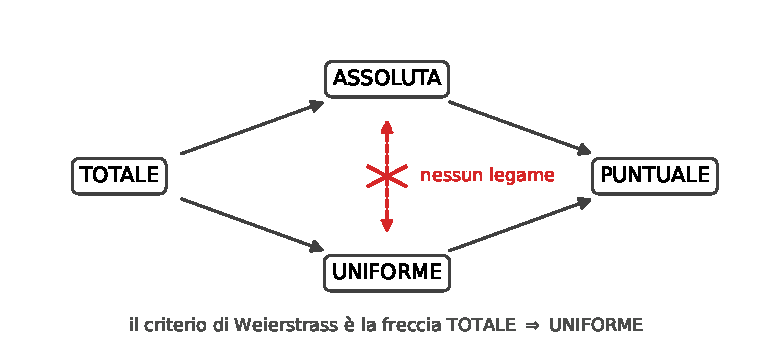
\includegraphics[width=0.7\linewidth]{figure/fig_09}
\caption{Relazioni fra i quattro tipi di convergenza per le serie di funzioni (schema
disegnato alla lavagna). Dalla convergenza totale si raggiunge la puntuale lungo due
``binari'' indipendenti; fra convergenza assoluta e convergenza uniforme non sussiste
alcuna implicazione.}
\label{fig:09}
\end{figure}

% [1:29:34]
\subsection{Teorema di integrazione per serie}

\paragraph{Teorema.} Sia $f_n:[a,b]\to\mathbb{R}$ continua per ogni $n\in\mathbb{N}$. Se
$\sum_{n=1}^{+\infty}f_n(x)$ converge uniformemente a $S(x)$ in $[a,b]$, allora
\begin{equation}
\sum_{n=1}^{+\infty}\int_a^b f_n(x)\,dx=\int_a^b\sum_{n=1}^{+\infty}f_n(x)\,dx
=\int_a^b S(x)\,dx .
\end{equation}

\paragraph{Dimostrazione.} Si considera la somma parziale $n$-esima della serie numerica a
primo membro:
\begin{align*}
I_n&=\int_a^b f_1(x)\,dx+\dots+\int_a^b f_n(x)\,dx\\
&=\int_a^b\big(f_1(x)+\dots+f_n(x)\big)\,dx=\int_a^b S_n(x)\,dx,
\end{align*}
dove si è usata la linearità dell'integrale. Per ipotesi $S_n\rightrightarrows S$ in
$[a,b]$ e ogni $S_n$ è continua (somma finita di funzioni continue), quindi si può passare
al limite sotto il segno di integrale:
\begin{equation}
\lim_{n\to+\infty}I_n=\lim_{n\to+\infty}\int_a^b S_n(x)\,dx
=\int_a^b\lim_{n\to+\infty}S_n(x)\,dx=\int_a^b S(x)\,dx . \qquad\blacksquare
\end{equation}

% [1:31:56]
\paragraph{In aula.} La dimostrazione è immediata una volta capiti i teoremi sulle
successioni: tutto consiste nel riconoscere che la somma parziale della serie degli
integrali è l'integrale della somma parziale. Si potrebbe premettere anche il teorema di
continuità del limite per dire che $S$ è continua — $S_n$ è somma di funzioni continue e
converge uniformemente — ma è così immediato che lo si usa direttamente.

% [1:35:44]
\paragraph{In aula (esercizio).} Allo stesso modo, dai teoremi sulle successioni di
funzioni si ricava il \emph{teorema di derivazione per serie}: la docente lo lascia da
scrivere come esercizio, dicendo che è ``la copia conforme'' dell'altro teorema, enunciato
sulle serie. Traccia: se $f_n\in C^1([a,b])$ per ogni $n$, se esiste $x_0\in[a,b]$ tale
che $\sum_n f_n(x_0)$ converge e se $\sum_n f_n'$ converge uniformemente in $[a,b]$,
allora $\sum_n f_n$ converge uniformemente a una somma $S\in C^1([a,b])$ e
\[
S'(x)=\sum_{n=1}^{+\infty}f_n'(x),\qquad x\in[a,b].
\]

% =====================================================================
% DUBBI:
%
% - Indici: su tutto il testo gli indici trascritti dall'OCR come "m" sono stati
%   normalizzati a "n" (indicazione esplicita). Fa eccezione il criterio di Cauchy,
%   dove servono due indici distinti n, m (audio [0:18:03]).
% - p.2 e p.3 degli appunti: il criterio di Cauchy è trascritto dall'OCR come
%   |f_n(x) - f(x)| < eps; è un errore di trascrizione, la quantità corretta è
%   |f_n(x) - f_m(x)| (audio [0:18:03] e [0:23:08]). Corretto nel testo.
% - p.1: "f è ricucibilmente continua" -> "f è sicuramente continua" (audio [0:02:50]).
% - p.1: "g'(eps) = g(eps)" -> derivata della funzione integrale di g uguale a g(x);
%   la variabile muta trascritta come epsilon è t.
% - p.4: l'OCR scrive sup |x|^{n+1}/(1-x) -> +infinito come se fosse un limite in n;
%   in realtà il sup su ]-1,1[ vale +infinito per ogni n fissato (audio [0:43:56]).
% - p.4: la riga "|x| < 1, per ogni M > 0, esiste eps > 0" è illeggibile; ricostruita
%   dall'audio [0:45:15] come restrizione ai compatti |x| <= r con 0 < r < 1.
% - p.5: "b.m.z." negli appunti è quasi certamente "Leibniz" (criterio per le serie a
%   segni alterni), confermato dall'audio [0:51:32].
% - p.5: la stima del resto è scritta come |S_n - S| < 1/(n+1); la forma generale usata
%   qui è |S_n - S| <= a_{n+1}, che nell'esempio dà (n+2)/(n+1)^2 (audio [0:53:57]).
% - p.6: nei criteri di Cauchy per le serie gli indici N e n sono mescolati; normalizzati
%   a n (resto f_{n+1} + ... + f_{n+p}, per ogni n > nu).
% - p.7: "esiste nu > 0" -> nu è un indice in N; "alpha_{n+1}" di p.8 è M_{n+1}.
% - p.8: "AB Bioma usato 2 volte il criterio di Cauchy" -> "Abbiamo usato 2 volte il
%   criterio di Cauchy".
% - Figure: le immagini figure/Analisi_II_p001_1.png, p001_2.png, p005_2.png,
%   p005_5.png sono loghi e segni decorativi degli appunti, non figure matematiche;
%   non ricostruite. L'unica figura ricostruita (fig_01) è lo schema dei "binari"
%   delle implicazioni fra i tipi di convergenza, effettivamente disegnato alla
%   lavagna [1:16:17].
% - Teorema di derivazione per serie: enunciato solo annunciato a lezione [1:35:44] e
%   lasciato per esercizio; la traccia riportata è la trasposizione alle serie del
%   teorema sulle successioni, da verificare con la dispensa della docente.
% - Note organizzative: la frase dell'audio [1:34:21] sulla prossima lezione ("lunedì")
%   è disturbata e non si capisce se sia una data di lezione o di ricevimento [?].
% - Audio [0:22:33]: accenno a uno strumento di registrazione/trascrizione usato in
%   aula; passaggio confuso, riportato solo nella sostanza [?].
% =====================================================================
